\section{The full path to full-path indexing}
\label{sec:rename}

Although zoning fixes rename performance in \betrfs, it has drawbacks.
The locality is not as good as full-path indexing because full-path indexing is
only maintained inside a zone.
More importantly, zoning imposes zone maintenance cost.
If an operation incurs a zone split or merge, the cost of the zone split or
merge is charged to that operation.
Thus, \betrfs may pay a significant amount of tax to zone maintenance on
workloads that have nothing to do with renames.
For example, in Tokubench that creates 10 million small files, the cumulative
throughput has a sudden 56.6\% drop when 2 million files are created because
of zoning splits (\betrfsThree in Figure~\ref{fig:toku10M}).

Our paper in FAST'18~\cite{betrfs4} presents \betrfsFour (\betrfsThree
contains only bug fixes) that introduces a new solution for renames.
The new solution, \rr, doesn't tax other operations and keeps full-path
indexing.
Unlike zoning, \rr works directly on the \bet.
\betrfs in the VFS layer simply calls \rr in ft-index to complete renames.

\subsection{Range-rename}

\Rr is based on the fact that the full-path indexing in \betrfs groups all
keys involved in a rename in a contiguous keyspace.
Thus, if there exists an isolated subtree that contains and only contains all
those related keys, we can move all the keys by moving
the subtree around with a pointer swing.

There are two obstacles in this approach:
\begin{itemize}
\item[-] Completely isolated subtrees are rare. \bets splits nodes evenly, so
  most of the time, pivots are not file or directory boundary keys;
\item[-] Keys in the subtree are not updated. They are still full-paths in the
  source.
\end{itemize}

\Rr addresses these two issues with {\bf tree surgery} and {\bf key lifting},
respectively.

\subsubsection{Tree surgery}

\begin{figure}
  \begin{subfigure}{.45\textwidth}
    \centering
    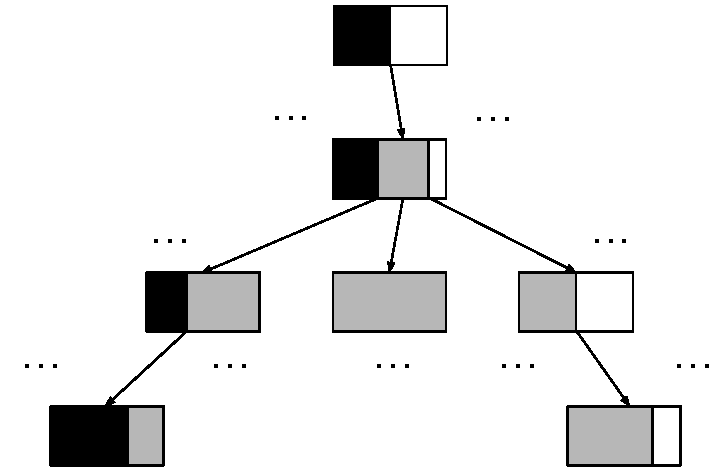
\includegraphics[width=.9\linewidth]{fig/slice-1}
    \caption{The original subtree contains /black, /gray and /white keys.}
    \label{subfig:slice-1}
  \end{subfigure}
  \begin{subfigure}{.45\textwidth}
    \centering
    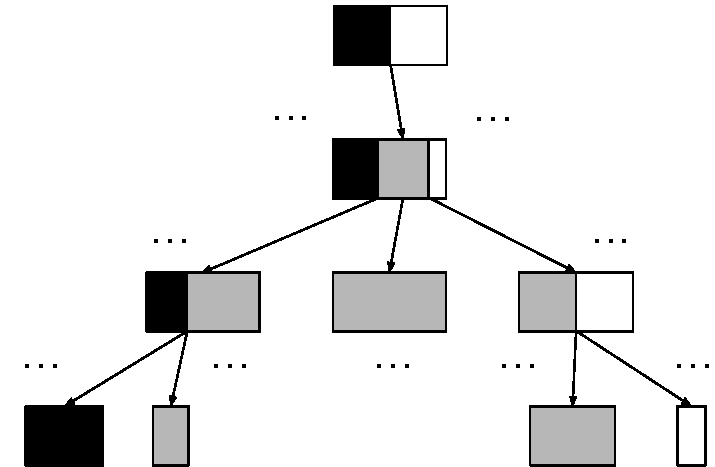
\includegraphics[width=.9\linewidth]{fig/slice-2}
    \caption{Slicing fringe leaves.}
    \label{subfig:slice-2}
  \end{subfigure}
  \begin{subfigure}{.45\textwidth}
    \centering
    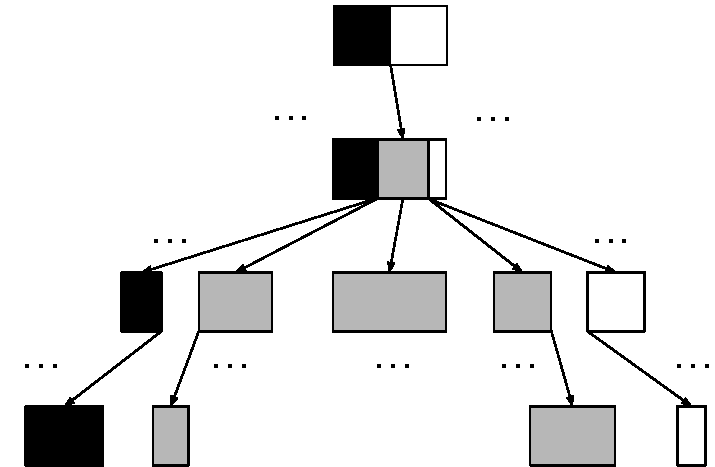
\includegraphics[width=.9\linewidth]{fig/slice-3}
    \caption{Slicing fringe nodes which were parents of fringe leaves.}
    \label{subfig:slice-3}
  \end{subfigure}
  \begin{subfigure}{.45\textwidth}
    \centering
    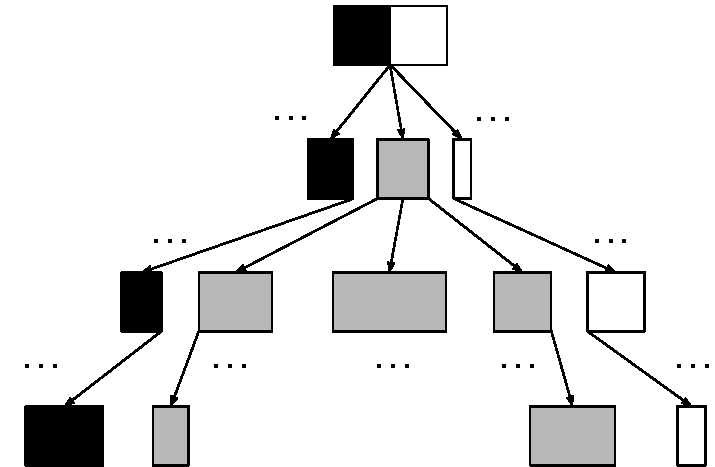
\includegraphics[width=.9\linewidth]{fig/slice-4}
    \caption{Slicing the LCA to get an isolated subtree of /gray keys.}
    \label{subfig:slice-4}
  \end{subfigure}
  \caption{Slicing /gray between /black and /white.}
  \label{fig:slice}
\end{figure}

Tree surgery slices out one isolated subtree in the source and another isolated
subtree in the destination, then uses a pointer swing to move the source
subtree to the destination.
The destination subtree needs to be sliced out because of two
reasons: 1. POSIX allows file renames to overwrite files, so there can be data
of the old file in the destination; 2. Because \bet injects new writes into the
root and flushes them down the tree gradually, some delete messages may not
reach their target key/value pairs,
which leaves deleted key/value pairs in the \bet.
Slicing in the destination also helps to setup pivots for the pointer swing.

Slicing can be viewed as getting an isolated subtree of range $(min, max)$.
Figure~\ref{fig:slice} shows how an isolated subtree of /gray keys are sliced
out.
Most nodes in the \bet either fall completely out of the range or completely
in the range.
Slicing only needs to deal with other nodes that are partly in the range and
partly out of the range, which are called {\bf fringe nodes}.

Fringe nodes can be identified by walking down the \bet with the $min$ and
$max$ keys.
This process results in two root-to-leaf path that contains all fringe nodes.
One important fringe node is the {\bf Lowest Common Ancestor (LCA)}, which is
the lowest node whose range covers both the $min$ and $max$ keys.
If the $min$ and $max$ keys lead to the same leaf node, that leaf is the LCA.
If the $min$ and $max$ keys diverge after the root, the root is the LCA.

After all fringe nodes are identified, slicing starts separating related keys
and unrelated keys from the bottom up until the LCA.
Slicing uses the already available tree mechanism, node splits, to accomplish
this job.
Unlike node splits in tree rebalancing that usually split the node evenly,
slicing splits the node with the $min$ or $max$ key.
A fringe node splits into two nodes, one fully in the range and the other fully
out of the range.
After the LCA is split, we get an isolated subtree and can move that subtree
around with a pointer swing.

Figure~\ref{fig:slice} shows how an isolated subtree is sliced out.
In this example, the slicing wants to get an isolated subtree that contains and
only contains /gray keys.
The original \bet is shown in Figure~\ref{subfig:slice-1}, all nodes that are
not completely gray are fringe nodes and the child of the root is the LCA.
The node split process starts in Figure~\ref{subfig:slice-2} where the leaves
are split.
At last, in Figure~\ref{subfig:slice-4}, the LCA is split and an isolated
subtree is formed.

One caveat here is that because we want to move the subtree around, all pending
messages above the LCA must be flushed at least to the LCA.
Therefore, slicing flushes pending messages down the tree while walking down
with the $min$ and $max$ keys.
In fact, during the walking, we flushed all messages to the leaves to make
node splits easier.

Another issue is that the \bet assumes all leaves to be at the same depth.
This means the source subtree and the destination subtree must be with the same
height.
To this end, when one slicing reaches its LCA, it needs to keep slicing until
the other slicing also reaches the LCA.

After the two subtrees are sliced out, tree surgery swaps the two subtrees with
pointer swings.
Ideally, the \bet can garbage collect the destination subtree immediately
because that tree will not be accessed anymore.
But there is no such out-of-the-tree garbage collection mechanism in
ft-index, so we swap the tree and let ft-index handle garbage
collection using its own cleaning mechanism.

The IO cost of tree surgery is $O(tree\ height)$ because 4 root-to-leaf walks
are performed, two in the source and two in the destination.
Compared to the old way that touches all related keys in $O(subtree\ size)$ IOs,
the cost of tree surgery is bounded by the height of the \bet and doesn't
grow infinitely when the size of the related data grows.

\subsubsection{Key lifting}

\begin{figure}
  \begin{subfigure}{.45\textwidth}
    \centering
    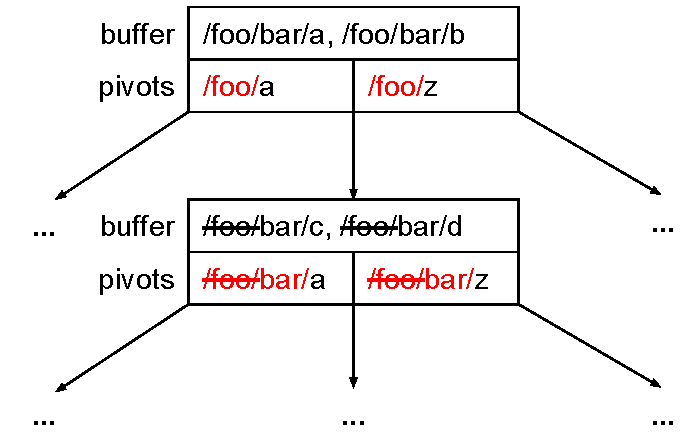
\includegraphics[width=.9\linewidth]{fig/lift-1}
    \caption{Keys in the subtree have /foo prefixes.}
    \label{subfig:lift-1}
  \end{subfigure}
  \begin{subfigure}{.45\textwidth}
    \centering
    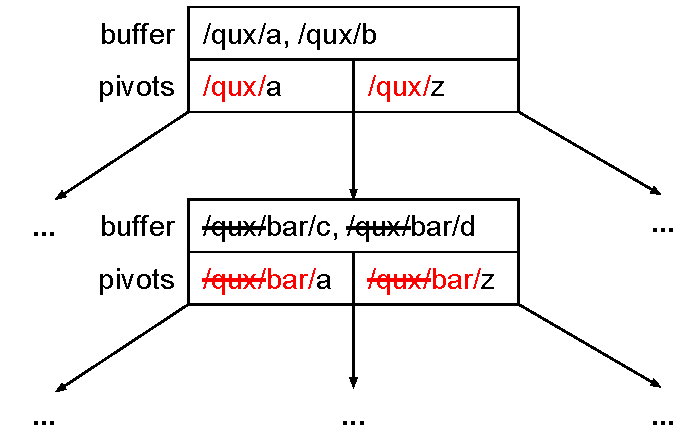
\includegraphics[width=.9\linewidth]{fig/lift-2}
    \caption{Keys int the subtree have /qux prefixes.}
    \label{subfig:lift-2}
  \end{subfigure}
  \caption{With key lifting, after moving the subtree to a new location, all
           prefix are updated automatically.}
  \label{fig:lift}
\end{figure}

After tree surgery, all keys in the subtree moved to the destination are still
full-paths in the source.
These keys must be updated to the new full-paths in the destination to make
the \bet correct.
A naive approach would traverse the subtree and update all keys.
This is costly and reverts the \rr back to the unbounded $O(subtree\ size)$.

Key lifting is introduced to deal with the key updating issue.
Key lifting is based on the observation that with certain key comparison
functions, the two pivots bounding a subtree in the parent restrict the prefixes
of keys in the subtree.
Specifically, \betrfs has \texttt{memcmp} as the key comparison function, so all
keys in the subtree must share the common prefix of the pivots.
This means that the common prefix is redundant information in the subtree and
only the suffixes of keys need to be stored in the subtree.

Key lifting converts \bets to lifted \bets.
All operations walking down a root-to-leaf path must collect lifted prefixes
along the way.
It needs to concatenate lifted prefixes and the suffix in the node to recover
the whole key.

An example can be seen in Figure~\ref{subfig:lift-1}, the common prefixes of
pivots are marked red in this figure.
In the parent, the common prefix of the two pivots is ``/foo/'', so we know all
keys follow that pointer must have that common prefix.
We use strikethrough to mark lifted prefixes.
These prefixes are not physically stored in the node, but virtually the keys are
perceived with these prefixes.

With key lifting, key updates complete automatically with tree surgery.
This is because now the prefix of keys in a subtree depends on the path from
the root to the subtree.
When the subtree is moved to a new location with tree surgery, the prefixes
of the keys in that subtree are changed according to the new location.

Figure~\ref{subfig:lift-2} shows the result of a subtree move.
The subtree used to be bounded by ``/foo/a'' and ``/foo/b'' in
Figure~\ref{subfig:lift-1}, so all keys were viewed with ``/foo/'' prefixes.
In the new location, the subtree is bounded by ``/qux/a'' and ``/qux/b'',
which means all keys in the subtree now have ``/qux'' prefixes.

Key lifting incurs no additional IO cost.
A root-to-leaf traversal just needs to collect lifted prefixes along the way,
and this doesn't add any IO cost.
To maintain key lifting, node splits or merges may need to modify keys because
pivots are added or removed.
But since node splits or merges already have to read all related nodes from
disk, no additional IO needs to be done.

Therefore, with lifting, key updates are done without IO cost during the tree
surgery process.
The total cost of \rr is still $O(tree\ height)$.

\subsection{Range-rename evaluation}

\begin{figure}[ht]
  \begin{tikzpicture}
    \begin{axis}[
      xlabel={Files created},
      ylabel={Throughput (files/sec)},
      xmin=0,
      xmax=10000000,
      xtick={0,2000000,4000000,6000000,8000000,10000000},
      xticklabels={0,2M,4M,6M,8M,10M},
      ymin=0,
      ymax=50000,
      scaled y ticks=false,
      mark repeat=50,
      grid=major,
      legend style={at={(1.1,0.5)},anchor=west},
      ]
      \addplot[
        color=black,
        line width=0.75pt,
        mark=*,
      ]
      file {./data/tokubench/betrfs4.csv};
      \addlegendentry{\betrfsFour}
      \addplot[
        color=gray,
        line width=0.75pt,
        mark=*,
      ]
      file {./data/tokubench/betrfs4-no-rr.csv};
      \addlegendentry{\betrfsFour-no-rr}
      \addplot[
        color=orange,
        line width=0.75pt,
        mark=*,
      ]
      file {./data/tokubench/betrfs3.csv};
      \addlegendentry{\betrfsThree}
      \addplot[
        color=red,
        line width=0.75pt,
        mark=pentagon*,
      ]
      file {./data/tokubench/btrfs.csv};
      \addlegendentry{Btrfs}
      \addplot[
        color=blue,
        line width=0.75pt,
        mark=triangle*,
      ]
      file {./data/tokubench/ext4.csv};
      \addlegendentry{ext4}
      \addplot[
        color=yellow,
        line width=0.75pt,
        mark=o,
      ]
      file {./data/tokubench/nilfs2.csv};
      \addlegendentry{nilfs2}
      \addplot[
        color=green,
        line width=0.75pt,
        mark=square*,
      ]
      file {./data/tokubench/xfs.csv};
      \addlegendentry{XFS}
      \addplot[
        color=purple,
        line width=0.75pt,
        mark=diamond*,
      ]
      file {./data/tokubench/zfs.csv};
      \addlegendentry{ZFS}
    \end{axis}
  \end{tikzpicture}
  \caption{Cumulative file creation throughput during the Tokubench benchmark.}
  \label{fig:toku10M}
\end{figure}

\begin{figure}[ht]
  \begin{tikzpicture}
    \begin{axis}[
      xlabel={File size (Bytes, log scale)},
      xlabel style={at={(0.5,-0.15)},anchor=north},
      ylabel={Throughput (renames/sec)},
      xmin=4096,
      xmax=67108864,
      xmode=log,
      xtick distance=2,
      log basis x=2,
      xtick={4096,8192,16384,32768,65516,131032,262064,524128,1048256,2096512,4193024,8386048,16772096,33544192,67088384},
      xticklabels={4KiB,8KiB,16KiB,32KiB,64KiB,128KiB,256KiB,512KiB,1MiB,2MiB,4MiB,8MiB,16MiB,32MiB,64MiB},
      xticklabel style={rotate=270,anchor=west},
      ymin=0,
      ymax=120,
      scaled y ticks=false,
      grid=major,
      legend style={at={(1.1,0.5)},anchor=west},
    ]
      \addplot[
        color=black,
        line width=0.75pt,
        mark=*,
      ]
      file {./data/rename/betrfs4.csv};
      \addlegendentry{\betrfsFour}
      \addplot[
        color=gray,
        line width=0.75pt,
        mark=*,
      ]
      file {./data/rename/betrfs4-no-rr.csv};
      \addlegendentry{\betrfsFour-no-rr}
      \addplot[
        color=orange,
        line width=0.75pt,
        mark=*,
      ]
      file {./data/rename/betrfs3.csv};
      \addlegendentry{\betrfsThree}
      \addplot[
        color=red,
        line width=0.75pt,
        mark=pentagon*,
      ]
      file {./data/rename/btrfs.csv};
      \addlegendentry{Btrfs}
      \addplot[
        color=blue,
        line width=0.75pt,
        mark=triangle*,
      ]
      file {./data/rename/ext4.csv};
      \addlegendentry{ext4}
      \addplot[
        color=yellow,
        line width=0.75pt,
        mark=o,
      ]
      file {./data/rename/nilfs2.csv};
      \addlegendentry{nilfs2}
      \addplot[
        color=green,
        line width=0.75pt,
        mark=square*,
      ]
      file {./data/rename/xfs.csv};
      \addlegendentry{XFS}
      \addplot[
        color=purple,
        line width=0.75pt,
        mark=diamond*,
      ]
      file {./data/rename/zfs.csv};
      \addlegendentry{ZFS}
    \end{axis}
  \end{tikzpicture}
  \caption{Rename throughput as a function of file size.}
  \label{fig:rename}
\end{figure}

\begin{table}[t]
  \centering
  \begin{tabular}{c | c c}
    \hline
    File system & find (sec) & grep (sec) \\
    \hline
    \hline
    betrfs 0.4  &  0.227  $\pm$  0.0 &  \xspace3.655  $\pm$ 0.1 \\
    betrfs 0.3  &  0.240  $\pm$  0.0 &  \xspace5.436  $\pm$  0.0 \\
    betrfs 0.4-no-rr  &  0.230  $\pm$  0.0  & \xspace3.600  $\pm$  0.1 \\
    Btrfs  &  1.311  $\pm$  0.1 &  \xspace8.068  $\pm$  1.6 \\
    ext4  &  2.333  $\pm$  0.1 &  42.526  $\pm$  5.2 \\
    nilfs2  &  6.841  $\pm$  0.1 &  \xspace8.399  $\pm$  0.2 \\
    XFS  &  6.542  $\pm$  0.4 &  \xspace58.040  $\pm$  12.2 \\
    ZFS  &  9.797  $\pm$  0.9 &  \xspace346.904  $\pm$  101.5 \\
    \hline
  \end{tabular}
  \caption{\label{tab:dirops} Time to perform recusive directory traversals of the Linux 3.11.10 source tree.}
\end{table}

We compare \betrfsFour with several file systems, including \betrfsThree,
\betrfsFour without \rr (as \betrfsFour-no-rr to represent \betrfsOne),
Btrfs~\cite{btrfs}, ext4~\cite{ext4}, nilfs2~\cite{nilfs2}, XFS~\cite{xfs}, and
ZFS~\cite{zfs}.
All benchmarks are run on a Dell Optiplex 790 with a 4-core 3.40 GHz i7 CPU, 4GB
RAM, and a 500 GB hard disk.

Figure~\ref{fig:toku10M} shows the result of TokuBench.
This benchmark creates 10 million files in a balanced tree directory where each
directory contains at most 128 files or subdirectories and measures the
cumulative throughput.
The performance of \betrfsThree plummets when about 2 million files are
created due to zone maintenance cost.
The instantaneous throughput remains between 200 to 600 files per second for 2
minutes, though it is more than 7000 files per second before and after that.
On the contrary, \betrfsFour is even faster than \betrfsOne (measured
as \betrfsFour-no-rr), probably because lifting eliminates long common
prefixes.
In all benchmarks we run, \betrfsFour doesn't show significant regression as
\betrfsThree with zoning does.

In Table~\ref{tab:dirops}, we measure locality by performance directory scans
(\texttt{find} and \texttt{grep}) in a linux-3.11.10 source directory.
\betrfsFour finishes much faster than other file systems except \betrfsThree
(5.77x faster in a find, and 2.21x faster in a grep).
Though \betrfsThree is still faster than other file systems with zoning, the
locality is not as good as full-path indexing file systems.

Figure~\ref{fig:rename} presents the result of our rename benchmark. In this
benchmark, we create a file and then rename it 100 times.
We measure the throughput of renames with different file sizes.
The performance of \betrfsOne keeps dropping as the file size grows larger.
However, \betrfsFour starts to use \rr when the file size is larger than the
node size in the \bet (4MB) and the performance is competitive with other file
systems.
But, because inode-based file systems finish a rename with a pointer swing in
$O(1)$ and \betrfsFour has a higher upper bound, the rename performance of
\betrfsFour is not always as good as other file systems.
